% Chapter 1

\chapter{Wprowadzenie} % Chapter title
%propedeutyka = «wiadomości wprowadzające do jakiejś dziedziny wiedzy» 
\label{ch:name} % For referencing the chapter elsewhere, use \autoref{ch:name}
 
\begin{flushright}
\emph{''Powszechnie wiadomo, że kamień potrafi myśleć. Na tym fakcie opiera się cała elektronika.''}

\textit{{\footnotesize (Równoumagicznienie, Terry Pratchett)}  }
\end{flushright}


Rozwój elektroniki, a szczególnie systemów mikroprocesorowych w ostatnich latach ma niebagatelny wpływ na niemal każdy aspekt naszego życia. Systemy te wraz z ewolucją są wykorzystywane już nie tylko do specjalnych zastosowań w wąskich dziedzinach, ale także jako elementy ułatwiające nam codzienne życie. Do jednych z wielu dziedzin, w których są kluczowe można zaliczyć min. : robotykę, motoryzację, medycynę, sport, tzw. inteligentne systemy. Obserwując zastosowania dzisiejszej elektroniki w obliczu społeczeństwa informacyjnego można stwierdzić trafność słów T. Pratchett'a. Powszechność elektroniki umożliwia jej obecność nawet w "kamieniach".

Pojęcie inteligentnych systemów w ostatnim czasie jest bardzo powszechne. Systemy te wyróżniają się tym, że zamiast wykonywania z góry założonego schematu działania są wyposażone w dodatkową inteligencję. Inteligencja ta daje dużo większe możliwości wykorzystania urządzenia, gdyż odpowiednio zastosowana daje możliwość odciążenia użytkownika z części zadań, lub nawet wykonania ich dużo sprawniej i dokładniej.
Jako, że wraz z rozwojem technologii możliwości układów SoC  wzrastają, przy niewielkich wciąż wymiarach, pozwala to zawrzeć w chipie module wiele podzespołów, takich jak  dedykowane układy graficzne, moduły komunikacji sieciowej, oraz inne podsystemy rozszerzające funkcjonalność układu.

Ponadto systemy wbudowane odgrywają znaczącą rolę szczególnie tam, gdzie niewielkie gabaryty urządzenia i niski pobór mocy są kluczowe.

Przykładem takiego systemu może być inteligenta kamera, której zadaniem jest detekcja  danego obiektu i podjęcie określonej przez projektanta akcji np. sterowania innym urządzeniem lub podzespołem, czy też tworzeniem statystyk.

\subsection*{Internet of Things}
Temat niniejszej pracy świetnie wpasowuje się w koncepcję tzw. Internetu Rzeczy (ang. Internet of Things- skr. IoT). Według której wszelkiego rodzaju urządzenia mogą stanowić jedną wielką sieć, pozwalającą sprawniej ze sobą wydajnie współpracować komunikując się ze sobą, wspólnie przetwarzając i wymieniając dane za pomocą sieci komputerowej.
Pod hasłem systemy inteligentne jak widać kryje się wiele różnych zagadnień, w których sprawne poruszanie się i umiejętność zintegrowania ich w jeden system jest dla projektanta kluczowe.

W niniejszej pracy zawarty jest opis projektu szybkiej inteligentnej kamery z interfejsem Ethernet, która wykrywa ludzi zbliżających się do niej, po czym otwiera drzwi i umieszcza wpis na serwerze http wraz z datą wykrycia i zdjęciem danej osoby.

\section{Przegląd dostępnych komercyjnych rozwiązań}

\begin{figure}[bth]
\centering
{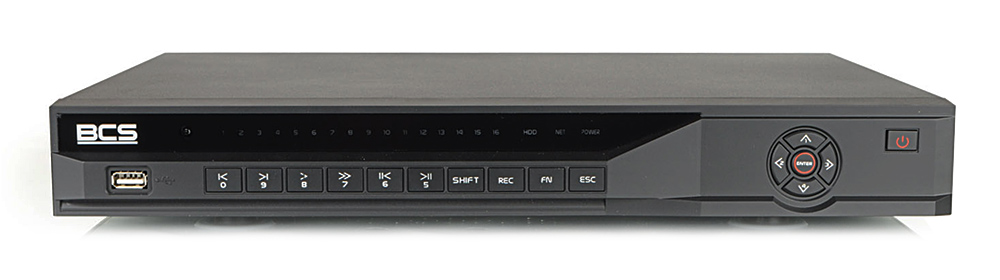
\includegraphics[width=0.8\linewidth]{gfx/bcs}}
\caption[Rejestrator BCS-NVT0802]{Rejestrator BCS-NVT0802.}
\label{fig:bcs}
\end{figure}

Prace techniczne i koncepcyjne poprzedziło badanie rynku. Za pomocą porównywarek cenowych zacząłem oceniać i porównywać oferty systemów monitoringu z różnych zakresów cenowych i jakościowych. Przyznaję, że w najniższej półce cenowej odnalazłem oferty o akceptowalnych parametrach. Jako przykład zostanie podany system monitorowania bezprzewodowego Conrad 8103J \ref{fig:bcs}, kameraIR, odbiornik 4-kanałowy. Producent zachwala rozwiązanie jako idealne do indywidualnego monitoringu wideo. W opisie produktu odnajdujemy informację, że komunikacja odbywa się po drodze radiowej, istnieje możliwość oglądania obrazu na ekranie monitora, oraz automatyczne diody podczerwieni umożliwiają transmisję czarno-białego obrazu w nocy.  Koszt zestawu wynosi 275 PLN.  

\begin{figure}[bth]
\centering
{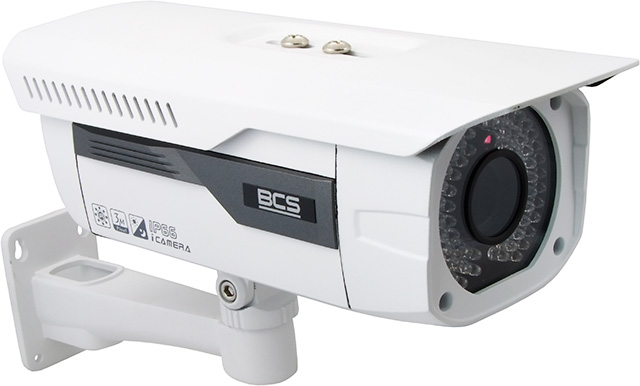
\includegraphics[width=0.6\linewidth]{gfx/bcsCam}}
\caption[ Kamera sieciowa BCS-TIP7300IR]{ Kamera sieciowa BCS-TIP7300IR.}
\label{fig:Chipscope}
\end{figure}

\begin{table}[b!]
%\myfloatalign
\caption[Conrad 8103J, kameraIR, odbiornik 4-kanałowy - dane i specyfikacja.]{Conrad 8103J, kameraIR, odbiornik 4-kanałowy - dane i specyfikacja.}
\begin{tabularx}{\textwidth}{|l|X|} 
 \hline
Dodatkowe światło IR & Tak \\ 
Komunikacja Analogowa, Radiowa Mikrofon &Tak \\
Napięcie robocze & 8 V/DC z zasilacza \\ 
Rodzaj kamery CCTV &  Bezprzewodowy system monitorujący \\
Rozdzielczość (TVL)& 720 x 480 p \\
Wymiary (odbiornik)& 24 x 78 x 107 mm \\  
Wymiary nadajnika & 26 x 35 mm \\ 
Zakres temperatury roboczej & od -10 do +50  C\\ 
Zasięg maksymalny & 100 m \\ \hline
\end{tabularx}  
\label{tab:compareAnalysers}
\end{table}

Z drugiej strony porównano rozbudowany system monitoringu IP: „Rejestrator BCS-NVR0802, 8 x Kamera BCS-TIP7300IR, Dysk 500GB, Akcesoria” firmy ivel electronics. Koszt zestawu 25 849,00 zł . W specyfikacji urządzania można odnaleźć bardzo wydajny sprzęt: 
Rejestrator BCS-NVR0802: 8 kanałowy sieciowy rejestrator cyfrowy z kompresją obrazu H.264, standard PAL. Nagrywanie do 8 kamer IP w D1 (25 kl/s), 720P (25 kl/s), 1080P (12 kl/s)



Prędkość zapisu rejestratora wynosi 200 klatek na sekundę (100 klatek w 1080P)
Wydajny procesor Dual-Core z systemem Embedded Linux, 8x Video, 8 x Audio, VGA, BNC, USB, HDMI, PTZ, RS485, Wyjścia/Wejścia alarmowe.
W rejestratorze można zamontować 2 dyski HDD SATA.
Możliwy podgląd przez internet na komputerze, smartfonie i tablecie. 

W zestawie jest też kamera sieciowa IP 3MPix FULL HD, 20 kl/s @3MPix (2048 x 1536), 25 kl/s @1080p. Przetwornik 1/2.8" SONY Progressive Scan CMOS. Obiektyw 8 - 16 mm/F1.6 CS Auto Iris, PoE, mechaniczny filtr podczerwieni. Zasięg podczerwieni 30 metrów. Hermetyczna  obudowa  klasy IP66 .

Po przeanalizowaniu dostępnych rozwiązań zaskakujący wniosek nasuwa się sam. Zauważamy sprzęt o bardzo dobrych parametrach, dostępny cenowo, ale niepraktyczny dla zwykłego użytkownika. Monitorując w dużej ilości zastosowań nie potrzebujemy nagrywać pełnometrażowego filmu z dużą dokładnością, który monitoruje obszar, w którym tak naprawdę niewiele się zmienia. Znacząca część zastosowań nie wymaga archiwizowania dużej ilości danych. Podgląd ze smartfona jest cennym dodatkiem aczkolwiek chcemy aby system sam informował o interesujących nas zdarzeniach i nie absorbował użytkownika w celu monitorowania obszaru. Konkluzją analizy dostępnych komercyjnych rozwiązań jest koncepcja zaprojektowania „Szybkiej, Inteligentnej kamery z interfejsem Ethernet”. Spośród istniejących rozwiązań kamera ma wyróżniać się właśnie na polu zastosowania. Tani wydajny sprzęt w połączeniu z algorytmami rozpoznawania obrazu możliwi opracowanie kamery bezkonkurencyjnej pod względem użyteczności, elastyczności zastosowania oraz pełnego wykorzystania potencjału sprzętowego.

\section{Przegląd dostępnych systemów wbudowanych}
Poniżej przedstawiono kilka z wielu dostępnych na rynku urządzeń, które mogą być zastosowane np. do rozwiązań typu „smart”.

Raspberry Pi 2 firmy Raspberry Pi Foundation jest minikomputerem wyposażonym w wydajną, 4-rdzeniową jednostkę SoC BCM 2836 firmy Broadcom. Posiada min.  złącze HDMI, 4 złącza USB i jedno Ethernet’owe. Ponadto kontroler kart SD, pozwala uruchomić system operacyjny z karty microSD. Płyta posiada także złącza dla dedykowanej kamery RaspiCam (sensor ov5xx) oraz złącze Display port, dla wyświetlacza. Cena : 175 zł

\begin{figure}[bth]
\centering
{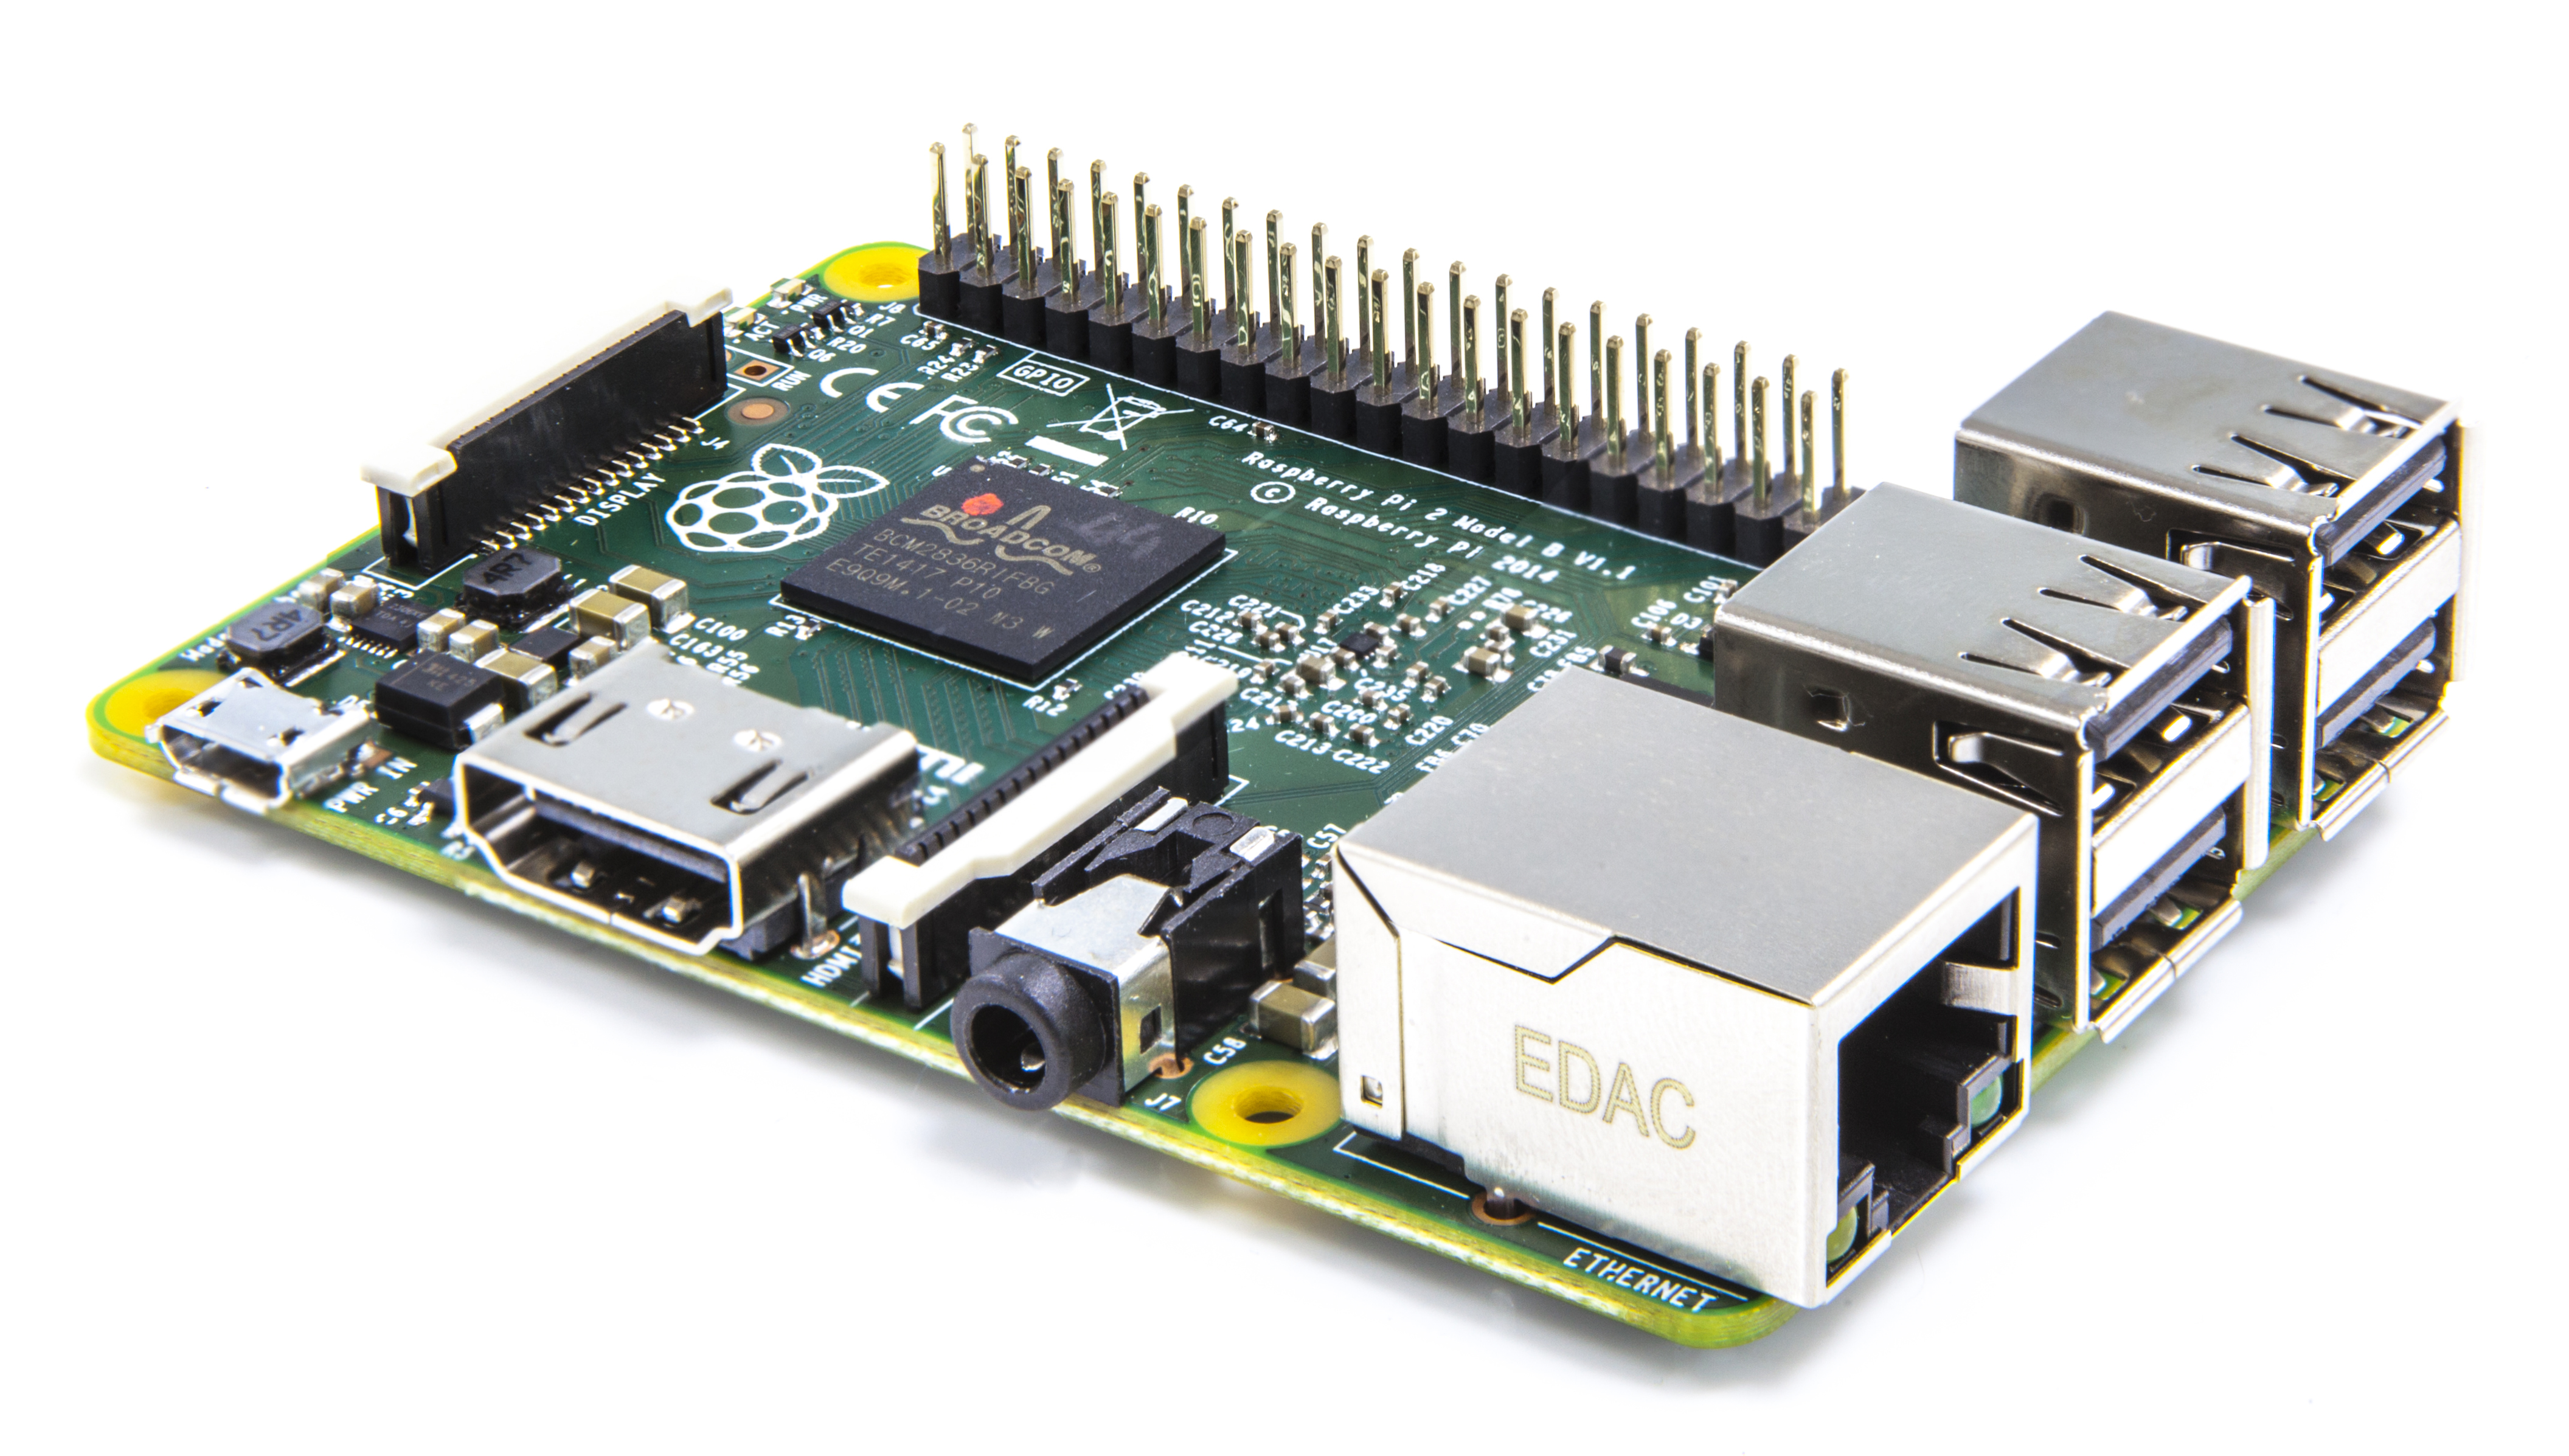
\includegraphics[width=0.8\linewidth]{gfx/rasp}}
\caption[Raspberry Pi w wersji 2]{Raspberry Pi w wersji 2}
\label{fig:Chipscope}
\end{figure}

BeagleBone Black Rev. C firmy BeagleBoard wyposażony w wydajny procesor Sitara AM335x firmy Texas Instruments taktowany zegarem 1GHz, 512 MB pamięci RAM i akcelerator grafiki 3D, a także złącza USB, HDMI i 92 porty GPIO. Cena: 249zł.

\begin{figure}[bth]
\centering
{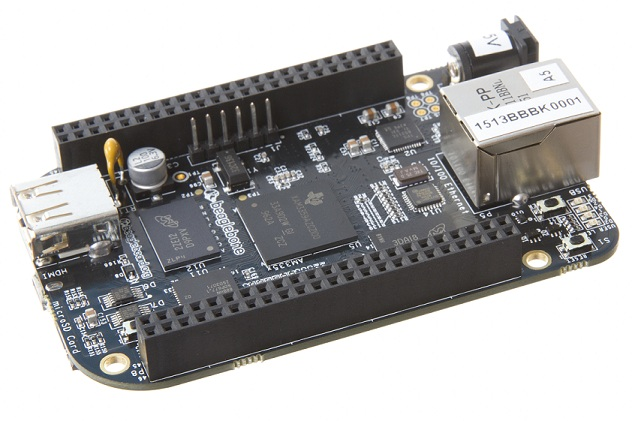
\includegraphics[width=0.8\linewidth]{gfx/beagle}}
\caption[BeagleBone Black Rev. C]{BeagleBone Black Rev. C}
\label{fig:Chipscope}
\end{figure}

OlinuXino Micro A13 firmy Olimex  z jednostką SoC Allwinner A13 i rdzeniem A13 Cortex A8 taktowanym zegarem 1GHz oraz jedostką GPU 3D Mali400 i 256 MB RAM stanowi tańszą alternatywę dla ww. urządzeń. Płyta posiada złącza USB, kontroler kart SD oraz wyjście VGA. Ponadto ma też osobne złącze dla wyświetlacza LCD i 40 portów GPIO. Cena: 35 EUR.

\begin{figure}[bth]
\centering
{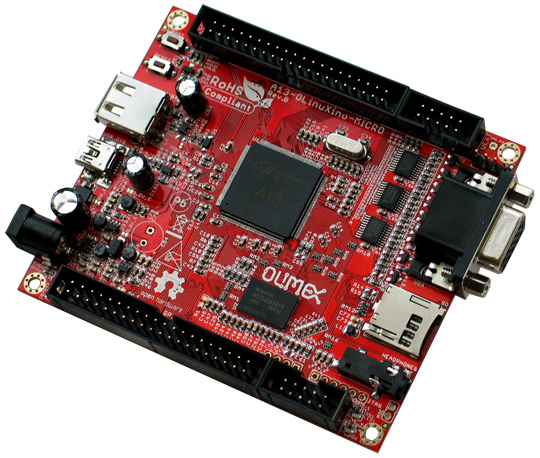
\includegraphics[width=0.6\linewidth]{gfx/olimex}}
\caption[OlinuXino Micro A13]{OlinuXino Micro A13}
\label{fig:Chipscope}
\end{figure}

Do zestawienia dodano rozwiązanie typowo z zastosowań przemysłowych: Wandboard Solo (model jednordzeniowy). Processor: Freescale i.MX6 Solo. Cores: Cortex-A9 Single core 
Graphic engine: Vivante GC 880 + Vivante GC 320. Memory: 512 MB DDR3. Warto wspomnieć o tym rozwiązaniu z powodu jego rosnącej popularności. Mały komputer jednopłytkowy wyróżnia solidne wykonanie, niezawodność oraz możliwość własnej adaptacji nakładek edm1 wykorzystującej standardowe złącze EDM. 

Do płytek nakładkowych typu edm (firmy Wandboard) lub rozwiązań SOM firmy olimex można opracować płytkę bazową, która będzie zinegrowana z kamerką i peryferiami komunikacji. Umożliwi to zmniejszenie rozmiaru, wykorzystanie tylko tych elementów, które są niezbędne. Zmniejszy to koszt projektu. Będziemy mieli również gwarancję, że jak zmieni się procesor będzie można wymienić płytkę nakładkową z procesorem (bez konieczności zmiany projektowej płytki bazowej).

Przyszłościowe koncepcyjne myślenie o rozwoju produktu skłoniło do wyboru dwóch rozwiązań, mniej popularnego tańszego układu firmy olimex i popularnych układów raspbery pi (z proc. BCM 2386). Oba wybrane zestawy demonstracyjne posiadają swoje odpowiedniki w płytach bazowych do rozwoju urządzeń tzw SOM (System on Module).

\begin{figure}[bth]
\centering
{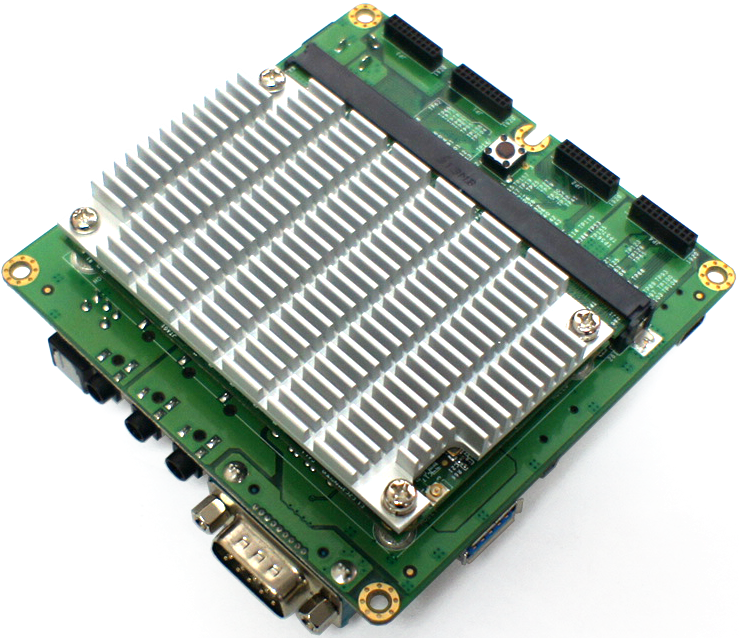
\includegraphics[width=0.6\linewidth]{gfx/wand}}
\caption[Wandboard]{Wandboard Solo}
\label{fig:Chipscope}
\end{figure}


\begin{table}[b!]
%\myfloatalign
\caption[Porównanie specyfikacji dostępnych rozwiązań.]{Porównanie specyfikacji dostępnych rozwiązań.}
\begin{tabularx}{\textwidth}{|lXXXXXX|} 
 \midrule
Urządzenie        & Procesor &Pamięć RAM & GPU & Interfejs kamery CSI & Ethernet & Cena \\
 \midrule
Raspberry Pi2       &  BCM 2386 900MHz quad-core ARM Cortex-A7 CPU &  1GB DDR2 SDRAM   &                     VideoCore IV &     Tak     &    10/100M  &  175 PLN\\
Beagle Bone Black Rev. C & AM335x 1GHz ARM Cortex-A8 & 512MB DDR3 RAM & PowerVR SGX530 & Nie & 10/100M & 249 PLN \\
OlinuXino Micro A13 & Allwinner A13 ARM Cortex A8 @1GHz & 256MB DDR2 RAM & 3D Mali400 & Tak & Nie (dostępny moduł USB-Ethernet)& 140 PLN \\
Wandboard Solo & Freescale i.MX6 Solo. & 512 MB DDR3 & Vivante GC 880 + Vivante GC 320 & ?? POSZUKASZ SAM ??? & 10/100M & 79 USD \\
\bottomrule
\end{tabularx}  
\label{tab:compareAnalysers}
\end{table}
%------------------------------------------------


\section{Architektura systemu Linux}
Obecnie Linux w systemach embedded \_ jest jednym z najpopularniejszych systemów operacyjnych. Dzięki uniwersalności i elastyczności można go spotkać w wielu urządzeniach dostępnych na rynku, takich jak : smartfony, tablety, odtwarzacze etc. Ważnym zagadnieniem w pracy z systemami opartymi na jądrze Linux jest znajomość jego architektury, a także połączenie wiedzy z  jego działania, administracji, konfiguracji oraz programowania w środowisku systemowym. W podrozdziale tym scharakteryzowane zostały podstawowe elementy każdego systemu opartego na jądrze Linux.

\begin{figure}[bth]
\centering
{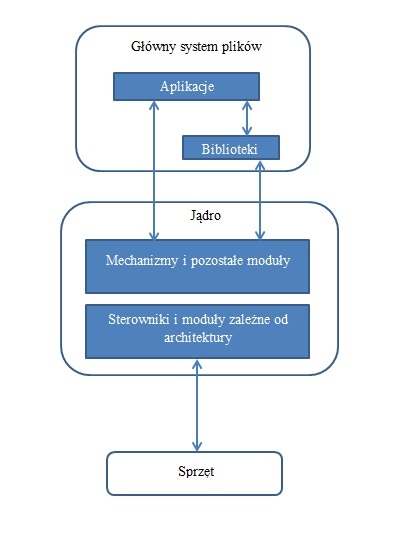
\includegraphics[width=0.7\linewidth]{sch/sch1}}
\caption[Architektura systemu Linux.]{Architektura systemu Linux.}
\label{fig:sch1}
\end{figure}

Jądro systemu – centralny element systemu operacyjnego, uprzywilejowany egzekutor zarządzający wszystkimi zasobami systemu. 

Moduły jądra – działają w uprzywilejowanym trybie; pozwalają na rozszerzanie funkcjonalności jądra bez ingerencji w kod źródłowy systemu.
Sterowniki – pośredniczą w komunikacji jądra ze sprzętem, oraz urządzeń wirtualnych (abstrakcyjnych)
Główny system plików – drzewo katalogów i plików

Biblioteki – używane przez niemal każdą aplikację; umożliwiają rozszerzenie funkcjonalności aplikacji działającej pod kontrolą systemu oraz stanowią interfejs do usług systemowych jądra.
Aplikacje – przenośne na poziomie kodu. Do podstawowych należą : powłoka, programy do operacji na plikach i katalogach, procesach, mechanizmach sieciowych, a także środowiska graficzne, kodery audio/wideo oraz wiele innych standardowych aplikacji.

\section{Dystrybucje systemu Linux}

Jako dystrybucję systemu Linux można określić kompletny system operacyjny, w skład którego oprócz samego jądra wchodzą dodatkowe usługi i aplikacje. To co odróżnia poszczególne dystrybucje, to jednolita organizacja plików konfiguracyjnych i mechanizm instalacji i zarządzania pakietami.
\begin{description}
\item Istnieje kilka kryteriów klasyfikacji dystrybucji:

\begin{itemize}[noitemsep]
\item Komercyjne lub niekomercyjne
\item Przeznaczone dla określonej grupy odbiorców : użytkowników zwykłych lub biznesowych
\item Wieloplatformowe, lub optymalizowane pod wybraną platformę sprzętową
\item Wyspecjalizowane lub ogólnego przeznaczenia
\item O określonym priorytecie np. przenośności czy bezpieczeństwa
\end{itemize}
\end{description}
\begin{description}
\item Wśród systemów wbudowanych opartych na platformie Raspberry można wyróżnić następujące dystrybucje:
	\begin{itemize}[noitemsep]
	\item Raspbian – najpopularniejsza dystrybucja, oparta na Debianie
	\item ArchLinux – pozwala w pełni dostosować system do wymagań użytkownika; pozbawiona GUI
	\item OpenELEC – dystrybucja typu Media Center
	\end{itemize}
\end{description}

W projekcie wykorzystana zostanie dystrybucja Raspbian .

\section{Konkurencyjne rozwiązania}

\begin{figure}[bth]
\centering
{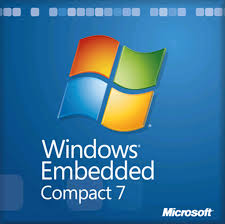
\includegraphics[width=0.3\linewidth]{sch/WE}}
\caption[Windows Embedded 7]{Windows Embedded 7}
\label{fig:sch1}
\end{figure}

Konkurencyjnym rozwiązaniem wchodzącym dynamicznie na rynek jest windows embedded.  Z każdą wersją obecnego systemu Windows udostępnia okrojoną wersję embedded. Rozwiązanie ma swoje zalety np. support techniczny, kompatybilność z aktualnymi desktopowymi systemami windows. Jako ciekawostkę można podać, że wymagania desktopowego systemu windows xp spełnia większość systemów wbudowanych, jak czyamy w wymaganiach systemu \footnote{https://support.microsoft.com/pl-pl/kb/314865}. Za wyborem linuxowego rozwiązania decydowało otwarte oprogramowanie, możliwość edycji ustawień systemowych z pozmiou kompilacji systemu. Pomijając indywidualne preferencje autora nie należy również zapominać, że systemy linux charakteryzują się bezpieczeństwem i jest to sprawdzone rozwiązanie dla systemów wbudowanych.

\section{Podsumowanie}
Na podstawie zestawienia popularnych systemów wbudowanych można stwierdzić, że każdy z nich oferuje różne konfiguracje i peryferia, co zmusza projektanta do optymalnego wyboru platformy sprzętowej pod kątem projektu. Analiza dostępnych urządzeń i dobranie optymalnego i niezawodnego rozwiązania stanowi ważny aspekt niniejszej pracy.
Najlepszy stosunek cena/jakość ma  Raspberry Pi 2. Czterordzeniowy procesor i 1GB pamięci RAM daje dużo większe możliwości względem konkurencyjnych produktów, co jest kluczowe przy  wymagających aplikacjach wykorzystujących przetwarzanie obrazu.
Jako dystrybucję systemu uruchamianą na płycie wybrano Raspbian.

